\section{Методы интеллектульаного анализа данных}

\subsection{Предмет интеллектуального анализа данных}

Интеллектуальный анализ данных (data mining) 
-- процесс выявления паттернов из больших объемов данных. \cite{curr}

Интеллектуальный анализ данных представляет собой междисциплинарную область,
в которой используются методы, идеи и принципы из следующих областей:
статистика, машинное обучение, распознавание образов,
вычислительная нейробиология, базы данных.
Стоит отметить, что данная область является частью более широкой области, 
которая называется выявление (обнаружение) знаний из баз данных (knowledge database discovery).
(zaki)

\begin{figure}[h]
    \center{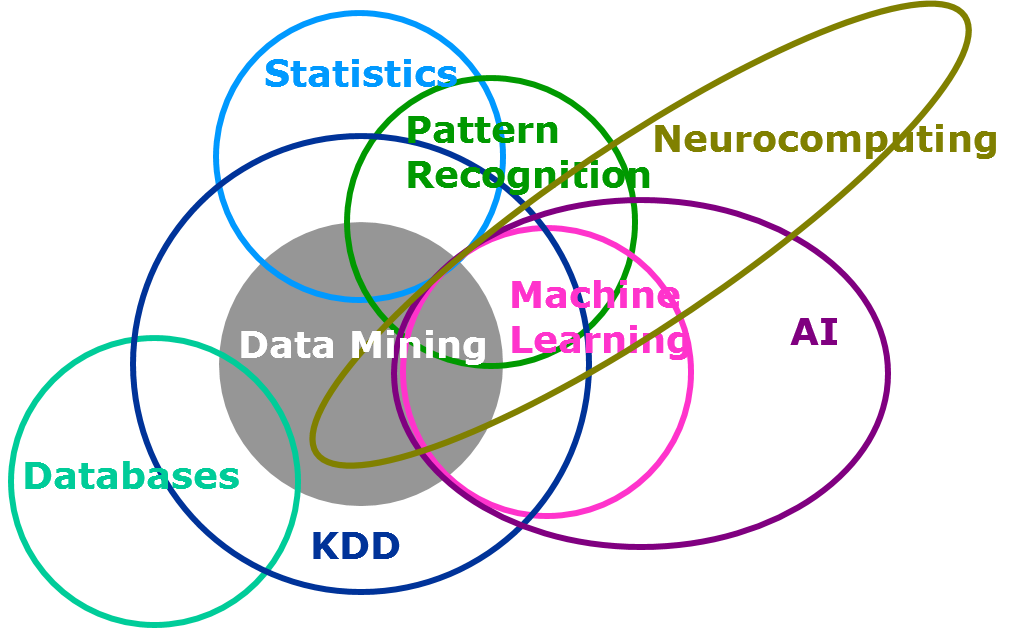
\includegraphics[width=10cm]{img/mining.png}}
    \caption{Место интеллектуального анализа данных среди других областей}
\end{figure}

Кроме этого, интеллектуальный анализ данных можно определить как часть
распознавания образов/паттернов (pattern recognition),
которая связана с обработкой данных из баз данных и выявлением паттернов, 
связанных с определенной предметной областью. (ссылка)
Сама область распознавания образов покрывает и другие области, например,
обработка сигналов и машинное зрение. (ссылка)

Опишем приведенные области, обозначим их основные идеи и принципы.

База данных -- организованная коллекция данных, которая собирается и хранится
при помощи компьютерных систем.
Для взаимодействия пользователя с базой данных используется
система управления базами данных (СУБД).

Теория баз данных поставляет формализованные методы и принципы проектирования и разработки баз данных и СУБД.
Обычно теоретически выделяют два главных типа построения баз данных: реляционные (SQL) и нереляционные базы данных (NoSQL).
Также иногда выделяют смешанный тип, появившейся сравнительно недавно:
новые реляционные базы данных, который совмещает лучшие
идеи и принципы из реляционных и нереляционных теорий и подходов (NewSQL). (ссылка)

В контексте интеллектуального анализа данных базы данных используются как источник данных.
Сами данные перед анализом обрабатываются, что также является частью процесса обнаружения знаний.
От типа и особенностей сбора и хранения данных в базе зависят последующие шаги анализа данных.

Данные можно представить в виде $n\times d$ матрицы данных:

\begin{equation} \label{data_matrix}
    \textbf{D} = 
    \begin{pmatrix}
    x_{1,1} & x_{1,2} & \cdots & x_{1,d} \\
    x_{2,1} & x_{2,2} & \cdots & x_{2,d} \\
    \vdots  & \vdots  & \ddots & \vdots  \\
    x_{n,1} & x_{n,2} & \cdots & x_{n,d} 
    \end{pmatrix}
\end{equation}

Вектор-строки вида:

\begin{equation}
    \textbf{x}_i = (x_{i,1}, ..., x_{i,d})
\end{equation}

в зависимсоти от предметной области имеют различные названия, например:
сущности, объекты, примеры и т.д.

Вектор-столбцы вида:

\begin{equation}
    \textbf{X}_j = (x_{1,j}, ..., x_{n,j})
\end{equation}

также могут иметь различные названия: атрибуты, свойства, переменные и т.д.

Обнаружение знаний из баз данных (knowledge database discovery, KDD) --  более широкая область
работы с данными из баз данных, частью которой является интеллектуальный анализ данных.
KDD определяют как процесс выявлений знаний (паттернов), который разбит на основные шаги: (ссылка)

\begin{enumerate}
    \item Селекция -- выборка данных из баз данных по определенным критериям;
    \item Обработка (pre-processing) -- приведение выбранных данных в подходящий вид 
    (очистка и удаление пропущенных значений, фиксирование атрибутов) для последующего анализа;
    \item Трансформация (transformation) -- трансформация данных в подходящую структуру данных, например, в матрицу данных \eqref{data_matrix};
    \item Интеллектуальный анализ данных (data mining) -- обнаружение паттернов в данных;
    \item Интерпретация и оценка (interpretation and evaluation).
\end{enumerate}

Следующим шагом также может быть использование, развертывание и эксплуатация обнаруженных знаний и паттернов для целей предметной области.
(ссылка)

Статистика, распознавание образов и машинное обучение являются поставщиками методов для каждого шага процесса KDD.
Каждая из этих областей имеет свои особенности, однако все они имеют также много общего.
Определим каждую область отдельно, выделим особенности и общие признаки.

\subsubsection{Теория статистики в контексте интеллекутального анализа данных}

Статистика -- дисциплина, сконцентрированная на сборе, организации, анализе, интерпретации и представлении данных. (ссылка)
Данная дисциплина является более общей, чем другие, так как ее идеи и методы в основном не зависят от предметной области,
а также имеют формализованную абстрактную форму в виде математической статистики и теории вероятностей.

В статистике выделяют следующие подобласти -- описательная статистика (descriptive statistics)
и статистический вывод (statistical inference).
Описательная (дескриптивная) статистика предоставляет методы обработки эмпирических данных,
систематизации и организации этих данных в определенном формате.
Статистический вывод предоставляет методы для вывода предположений об особенностях генеральной совокупности на основе выборки.
(ссылка)

В статистическом выводе выделяют два подхода -- частотный и байесовский походы. (ссылка)
Два данных подхода сложились из двух различных интерпретаций вероятности, основанные на объективных доказательствах
и субъективных степенях веры. Частотный подход следует из определения вероятности через частоту появления
из общего множества элементарных событий. Байесовский подход опирается на понятия априорной и апостериорной вероятности.
Априорная вероятность -- это такая вероятность, которая определена и известна до учета новых данных.
Апостериорная вероятность -- вероятность, которая определяется после поступления новых данных.
В контексте интеллектуального анализа данных оба подхода применяются и комбинируются
на основе критериев, определяемых через требования предметной области к выбранной статистической модели.

Статистика формализуется на основе математики через математическую статистику и теорию вероятностей.
Коротко опишем терминологию из этих областей математики, которую будет использовать в дальнейшем.

Математическая статистика использует основы теории вероятности, а именно понятия случайной величины и вероятностного распределения.

Вероятностное пространство -- измеримое пространство, состоящее из тройки:

\begin{equation}
    (\Omega, F, P )
\end{equation}

где $\Omega$ -- множество элементарных событий, например, всех возможных исходов эксперимента;
$F$ -- пространство событий, которые сами состоят из элементарных событий, имеет структуру $\sigma$-алгебры;
$P$ -- вероятностная мера, определенное как отображение $P: F\rightarrow [0,1]$, которое удовлетворяет свойствам вероятности.

Случайной величиной называется измеримое отображение из пространства элементарных событий в множество вещественных чисел:

\begin{equation}
    X: \Omega \rightarrow \mathbb{R}
\end{equation}

Обобщением случайной величины является понятие случайного элемента, которая определяется как отображение
из пространства элементарных событий в какое-либо измеримое пространство.

Выделяют три вида случайных величин:

\begin{itemize}
    \item Дискретная случайная величина -- случайная величина, которая имеет дискретные выходные данные и значения;
    \item Непрерывная случайная величина -- случайная величина, имеет значения на каком-либо непрерывном промежутке;
    \item Смешанная случайная величина -- имеет свойства дискретной и непрерывной.
\end{itemize}

(Определение pmf, pdf, cdf)

Существует большое количество видов распределений, каждое их которых имеют свою особую роль в математической статистике.

(Работа с двумя с.в., зависимость и независимость, услования вероятность, теорема байеса, совместное распределение)

(Многомерный анализ, проклятье размерности)

(Ядерные методы)

(Выборка, гипотезы, выбор статистической модели (model selection), оценка параметров, интервалы)

(Сравнение частотного и байесовского подхода на основе математической статистики)

В итоге можно сказать, что статистика является подобием теоретического фреймфорка для каких-то определенных предметных областей.
Интеллектуальный анализ данных зависит от предметной области, однако в нем удачно используются статистические методы.


\subsubsection{Искуственный интеллект и интеллекутальный анализ данных}


(Искуственный интеллект -- основные принципы)

(Машинное обучение -- в основном про предсказания)
(Классификация, регрессия, ранжирование, кластеризация, сокращение размерности и manifold learning)

(Термины: примеры (инстансы), фичи(атрибуты), лейблы, гиперпараметры (AutoML), обучающая выборка, валидационная выборка, 
тестовая выборка, функции потерь, множество гипотез)

(Переобучение, недообучение)

(Все модели ошибаются, бесплатных обедов не бывает)

(Обучение с учителем, обучение без учителя, частичное обучение с учителем, трансдуктивный вывод, онлайн обучение, обучение с подкреплением
активное обучение)

(Глубокое обучение)

(Байесовский подход)

(Эволюционный поход)

(Место вычислительной нейробиологии и связь с интеллектуальным анализом данных)

(Место распознавания образов и связь с data mining)


\subsection{Анализ временных рядов и предсказательный вывод}

(Определение временных рядов, случайные процессы)

(Определение предсказаний)

Выделяют следующие этапы предсказательного вывода:

\begin{enumerate}
    \item Определение проблем и задач
    \item Сбор данных
    \item Выбор моделей
    \item Проверка моделей
    \item Разворачивание модели
    \item Мониторинг производительности модели прогнозирования
\end{enumerate}


(Описание этапов)

(Очистка данных. Импутация данных. )

(Спектральный анализ и вейвлет анализ)

(Автокорреляция и кросс-корреляция)

\subsection{Сравнительный анализ методов}

(Регрессия)

(Кластеризация)


\subsection{Выбор метода и его обоснование}

(K-shape)

\clearpage